\section{Introduction}
<<<<<<< HEAD
\label{sec:introtduction}
Our Task in this internship was to find a machine learning method to control a robot arm such that robot arm throw a object in form of a cylinder as far as possible from his original position. For this experimental task we got a Gazebo environment with a Table, a Hollie robot arm who was fixed on the table, a cylinder to throw and a camera which points on the cylinder, see Fig. \ref{init_state}.
As the focus in this internship was in neurorobotics we chose to use spiking neural network(SNN) as machine learning method. The goal was now to find a suitable learning algorithm for a spiking neuronal network which could solve the task. We came to the conclusion that a reinforcement learning algorithm was the best way to let the network learn and after search of reinforcement algorithms we diced to use evolutionary Algorithms. 
To design a spiking neuronal network we used the neurorobotic platform. It's a platform specialized for develop and train spiking neuronal networks. For that the platform includes the following things:
=======
The goal of this course was to teach a simulated robot arm to throw an object (in our case a blue cylinder) as far as it is possible within the given simulation. The simulation in this case ran in the Neurorobotics Platform (NRP) which utilizes the Robotic Simulator Gazebo and the spiking neural network simulator nest.\\%hier evtl. noch Weblinks zu NEST NRP GAZEBO 
The Experimental setup consisted of a table on which a HoLLiE robot arm and a blue cylinder were placed.
The initial setup can be seen in Fig. \ref{init_state}. For every iteration in the simulation the cylinder was placed at the exact same position. 
As the focus in this course was neurorobtics we used spiking neural networks as the basis of our machine learning approach.  
The goal was to find a suitable learning algorithm for a spiking neuronal network which could solve the task. We chose a reinforcement learning approach in combination with an evolutionary strategy to adjust the weights of the network.
For the simulation and design of the spiking neural network we used NRP including the SNN simulator NEST. For that the platform includes the following things:
>>>>>>> 32d0de4ac4ce6b832b85dd8c8628ff556a18aad4
 \begin{itemize}
\item a Gazebo environment and simulation
\item editors to create transfer functions to control the actors and get sensor data
\item a editor to create the neurons and synapses of the network
\item a view output mechanism to monitor the simulation
\item a so called virtual coach configure and start simulations for the learning task.
\end{itemize} 
\begin{figure}[H]
	\centering
	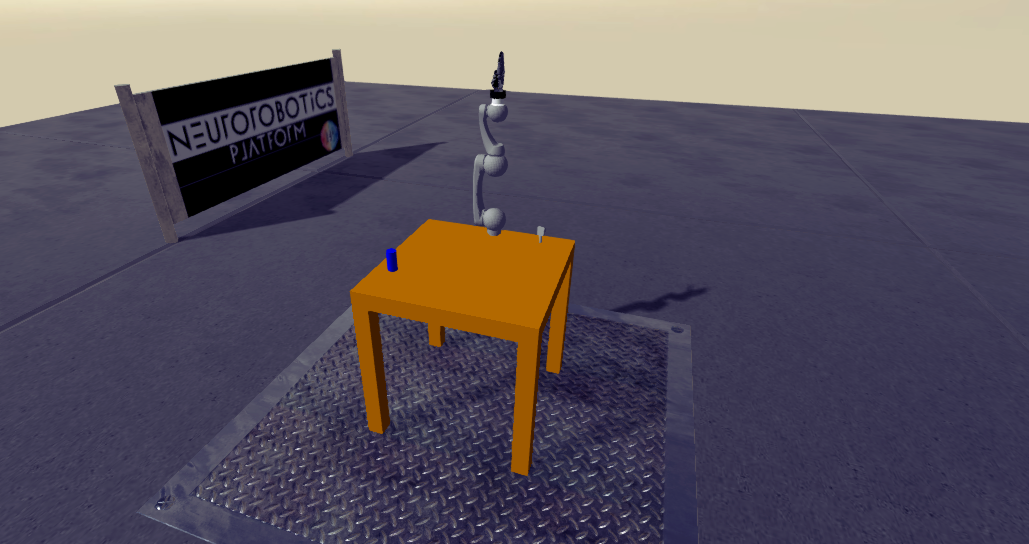
\includegraphics[width=2.2in]{img/init_state.png}
	\DeclareGraphicsExtensions.
	\caption{General task environment with inital state }
	\label{init_state}
\end{figure}
<<<<<<< HEAD
\section{Related Work}
As we use Reinforcement Learning and spiking neuronal networks we do here a short instruction to them.
\subsection{Reinforcement Learning}
Reinforcement Learning is based on the interaction of a agent (in our case the robot arm) with his environment (in our case Gazebo). To Learn, the agent get for every action in a state a reward(distance) - depending on if the action was good or not(far or short distance)- and a new state. If the action in the corresponded state got a high reward, then it's more likely that the actor uses the same action next time he is in this state again. To see a simple illustration of the whole learning process see Fig. \ref{re_base}
=======

\section{Related Work}%muss noch korrigiert werden
As we use Reinforcment Learning and spiking neuronal networks we do here a short instruction to them.
\subsection{Reinforcment Learning}%muss noch korrigiert werden
Reinforcment Learning is based on the interaction of a agent (in our case the robot arm) with his environment (in our case Gazebo). To Learn, the agent get for every action in a state a reward(distance) - depending on if the action was good or not(far or short distance)- and a new state. If the action in the corresponded state got a high reward, then it's more likeliky that the actor uses the same action next time he is in this state again. To see a simple illustration of the whole learning process see Fig. \ref{re_base}
>>>>>>> 32d0de4ac4ce6b832b85dd8c8628ff556a18aad4
\begin{figure}[H]
	\centering
	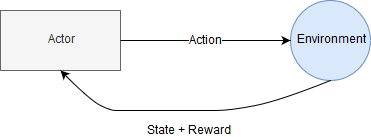
\includegraphics[width=2.2in]{img/re_base.png}
	\DeclareGraphicsExtensions.
	\caption{General illustration of reinforcement learning}
	\label{re_base}
\end{figure}

<<<<<<< HEAD
\subsection{Spiking Neuronal Networks}
Spiking neuronal networks is a variant of artificial neuronal(ANN) networks which are closer to the human brain as model then other ANN. In SNN the information isn't represented by the output value of a neuron, as spikes of a single neuron always looks the same, it's represented in the timing a neuron spikes. For example the information can be represented by the difference from the present spike to the last spike. To learn, there are, as in other ANN's weights which describes how much a output spike of a previous neuron influence the next neuron in order. To train the SNN u have to adept this weights, which is quiet difficult as there is no activation function like in standard ANNs. Compared to other ANNs in SNNs each neuron got a activation potential and every time this got exceeded the neuron spikes with a predefined spike.
=======
\subsection{Spiking Neuronal Networks}%muss noch korrigiert werden
Spiking neuronal networks is a variant of artifical neuronal(ANN) networks which are closer to the human brain as model then other ANN. In SNN the information isn't represented by the autoput value of a neuron, as spikes of a single neuron always looks the same, it's represented in the timing a neuron spikes. For example the information can be represented by the difference from the present spike to the last spike. To learn, there are, as in other ANN's weights which describes how much a output spike of a previous neuron influence the next neuron in order. To train the SNN u have to adept this weights, which is quiet difficult as there is no activation function like in standard ANNs. Compared to other ANNs in SNNs each neuron got a activation potential and every time this got exceeded the neuron spikes with a predefined spike.
>>>>>>> 32d0de4ac4ce6b832b85dd8c8628ff556a18aad4

\section{Throwing Challenge}
\subsection{Task}
As said our Task in this internship was to throw a cylinder as far as possible form a table. For this the experiment we got the following sequence of events.
 \begin{itemize}
\item State 1 initial state: The robot arm and the cylinder are in their original state, see Fig. \ref{init_state}.
\item State 2 throwing state: The robot arm move to the cylinder to throw or bump him away as far as possible. If the cylinder lands on the ground or 20 sec are over go back to state 1.
\end{itemize}
Our goal was now to optimize the robot moves in state 2 with a SNN. For that we had to control 7 parameters with a SNN, 6 for the angles of the robot arm + 1 for open and close the hand. 
To achieve the goal we decided to divide our tasks in 3 smaller Task:
 \begin{itemize}
\item 1. Approach the Cylinder
\item 2. Grab the Cylinder
\item 3. Throw the Cylinder
\end{itemize}
In the End of our internship the task 1 and 2 were hard coded and task 3 was achieved with a SNN.
\subsection{Challenges}
\label{sec:challenges}
While the internship we encountered with a view problems. The most important were:
 \begin{itemize}
\item The Gazebo simulation got a non deterministic behaviour so it was hard to find good weights for the SNN, as it was hard to reproduce the same behaviour with the same weights
\item Gripping the Cylinder with the hand. Trough non deterministic behaviour of the simulation it was possible that sometimes the hand didn't grab the cylinder although it grabbed the cylinder many times before with the same joint configuration. This could led to inaccurate results in training, as our precondition in training was that the robot grabbed the cylinder.
\item Exploding hand, sometimes the hand just exploding and the cylinder bugged away this lead to unrealistic high distances.
\item The Distance measurement wasn't really accurate, sometimes we a achieved big distance with small throws.
\end{itemize}


